\documentclass[12pt]{article}
\usepackage[a4paper, total={6in, 8.5in}]{geometry}
\usepackage{graphicx}
\graphicspath{ {images/output/} }
\usepackage{amsmath}
\usepackage{minted}
\usepackage{multicol}
\usepackage{caption}
\usepackage[english]{babel}
\usepackage{placeins}
\usepackage{titling}


\begin{document}
\vspace*{\fill}
\begin{center}

    \emph{Heaven's Light is Our Guide} \\
    \textbf{Rajshahi University of Engineering and Technology} \\

    \begin{figure}[H]
        \centering
        
\includegraphics[scale=.34]{images/RUET_logo.png}
        \label{fig:ruet_logo}
    \end{figure}
    \vspace{5mm}

    \textbf{Course Code}\\
    ECE 3112\\
    \vspace{3mm}
    \textbf{Course Title}\\
    Microprocessor, Assembly Language \& Interfacing Sessional

    \vspace{5mm}
    \textbf{Experiment Date:} {May 25, 2024},\\
    \textbf{Submission Date:} {June 3, 2024}\\

    \vspace{5mm}
    \textbf{Lab Report 6: Using Assembly Language to Program 8086 Microprocessor to Solve Problems Related To Shifting \& Stack.}

    \vspace{15mm}

    \begin{tabular}{c|c}
        \textbf{Submitted to} & \textbf{Submitted by} \\
        Md. Omaer Faruq Goni  & Md. Tajim An Noor     \\
        Lecturer              & Roll: 2010025         \\
        Dept of ECE, Ruet     &                       \\
    \end{tabular}

\end{center}
\vspace*{\fill}

\clearpage
\title{Problem 6.1}
\author{}
\date{}
\maketitle

\section*{Problem Description}
Write a code to take two input from user as Binary and multiply them using shifting operation and output the result in binary.

\section*{Tools Used}
\begin{itemize}
    \item emu8086 - 8086 Microprocessor Emulator
    \item MacTeX -\LaTeX  compiler.
    \item VS Code with \LaTeX workshop extension as a text editor.
\end{itemize}

\section*{Process}
\subsection*{Code:}

\begin{multicols}{2}{|}
    \begin{minted}[linenos,breaklines,breakanywhere]{nasm}
DATA SEGMENT
    INA DW ?
    INB DW ?   
    COUNT DB 16
DATA ENDS

CODE SEGMENT
    ASSUME CS:CODE,DS:DATA
    
MAIN PROC
    MOV AX,DATA
    MOV DS,AX    
    
    CALL MULTIPLY
    CALL BIN_OUT
    
    MOV AH, 4CH
    INT 21H
MAIN ENDP
    
MULTIPLY PROC
    CALL BIN_IN
    MOV INA, CX
    CALL BIN_IN
    MOV INB, CX
    
    MOV AX, INA
    MOV BX, INB
    PUSH AX
    PUSH BX
    XOR DX, DX
    
    LOOP_:
        TEST BX, 1
        JZ END_IF
        
        ADD DX, AX
        
    END_IF:
        SHL AX, 1
        SHR BX, 1
        
        JNZ LOOP_
        POP AX
        POP BX
        
        RET           
MULTIPLY ENDP

BIN_IN PROC
    XOR BX, BX
    MOV AH, 1
    INT 21H  
        
    INPUT:
        CMP AL, 0DH
        JE EXIT_
        
        AND AL, 0FH
        SHL BX, 1
        OR BL, AL
        
        INT 21H       
        JMP INPUT
        
    EXIT_:
        MOV DL, 0DH
        MOV AH, 2
        INT 21H
        MOV DL, 0AH
        INT 21H
        
        MOV CX, BX
        RET       
BIN_IN ENDP 

BIN_OUT PROC
    MOV BX, DX
        
    PRINT:
            RCL BX, 1
            JC PRINT1
            JNC PRINT0
            
    PRINT1:
        CMP COUNT, 0
        JE END_
            
        MOV DL, '1'
        MOV AH, 2
        INT 21H
        DEC COUNT
        JMP PRINT
            
    PRINT0:
        CMP COUNT, 0
        JE END_ 
            
        MOV DL, '0'
        MOV AH, 2
        INT 21H
        DEC COUNT
        JMP PRINT
        
    END_:
        RET            
            
BIN_OUT ENDP

END MAIN
    \end{minted}
\end{multicols}


\subsection*{Output}
\begin{center}
    \centering
    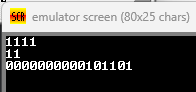
\includegraphics[width = .4\textwidth]{MUL.png}
    \captionof{figure}{Binary input \& output}
\end{center}


\clearpage
\title{Problem 6.2}
\author{}
\date{}
\maketitle

\section*{Problem Description}
Write a code to take input from user as string and then out the string in reverse. Use stack.

\section*{Process}
\subsection*{Code:}

\begin{multicols}{2}{|}
    \begin{minted}[linenos,breaklines,breakanywhere]{nasm}
DATA SEGMENT

DATA ENDS
CODE SEGMENT
    ASSUME CS:CODE, DS:DATA
    
START:
    MOV AX, DATA
    MOV DS, AX
    
    XOR CX, CX
    MOV AH, 1
    INT 21H
    
INPUT:
    CMP AL, 0DH
    JE EXIT_
    
    PUSH AX
    INC CX
    
    INT 21H
    JMP INPUT     
    
EXIT_:   
    MOV AH, 2
    MOV DL, 0DH
    INT 21H
    MOV DL, 0AH
    INT 21H
    
OUTPUT:
    POP DX
    INT 21H
    LOOP OUTPUT
     
CODE ENDS
END START  
\end{minted}
\end{multicols}

\subsection*{Output}
\begin{center}
    \centering
    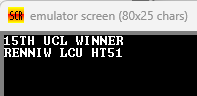
\includegraphics[width = .4\textwidth]{stkRev.png}
    \captionof{figure}{Hexadecimal input \& output}
\end{center}



\clearpage
\title{Problem 6.2}
\author{}
\date{}
\maketitle

\section*{Problem Description}
Write a program that lets the user type some text, consisting of words separated by blanks, ending with a carriage return, and displays  the text in same word order as entered, "this is a test" becomes "siht si a tset".

\section*{Process}
\subsection*{Code:}

\begin{multicols}{2}{|}
    \begin{minted}[linenos,breaklines,breakanywhere]{nasm}
DATA SEGMENT
    COUNT DW 0
DATA ENDS

CODE SEGMENT
    ASSUME CS:CODE, DS:DATA

START:
    MOV AX, DATA
    MOV DS, AX
    
    XOR CX,CX
    
    MOV AH, 1
    INT 21H

INPUT:
    CMP AL, 0DH
    JE END_
    
    PUSH AX
    INC CX
    INT 21H
    JMP INPUT

END_:
    MOV DX, 0DH
    MOV AH, 2
    INT 21H
    MOV DX, 0AH
    INT 21H
    
    MOV BX, SP
    SUB BX, CX
    SUB BX, CX
    
    XCHG BX, SP
    PUSH 20H
    XCHG BX, SP
    INC COUNT
        
TO_NEW_STK:
    POP DX
    XCHG BX, SP
    PUSH DX
    XCHG BX, SP
    INC COUNT       
    
    LOOP TO_NEW_STK

    MOV CX, COUNT
    MOV COUNT, 0
    PUSH 20H
    INC COUNT 

REVERSE:
    XCHG BX, SP
    POP DX 
    
    XCHG BX, SP
    CMP DL, 20H
    
    JNE SKIP
    
    MOV AH, 2

REV_PRINT:
    POP DX
    INT 21H
    
    DEC COUNT
    JNZ REV_PRINT
    
    MOV DX, 20H

SKIP:
    PUSH DX
    INC COUNT
    
    LOOP REVERSE
    
    MOV AH, 4CH
    INT 21H

CODE ENDS
END START
\end{minted}
\end{multicols}

\subsection*{Output}
\begin{center}
    \centering
    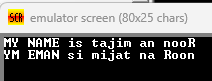
\includegraphics[width = .4\textwidth]{sentRev.png}
    \captionof{figure}{Hexadecimal input \& output}
\end{center}




\pagebreak
\section*{Keywords}
These are the new keywords learned while solving the Problems
\begin{description}
    \item[PUSH] Used to put a word at the top of the stack.
    \item[POP] Used to get a word from the top of the stack to the provided location.
    \item[XCHG] Used to exchange the data from two locations.
    \item[CALL] Used to call a procedure and save their return address to the stack.
    \item[RET] Used to return from the procedure to the main program.
\end{description}

\end{document}
